%   DOCUMENT CLASS  %%%%%%%%%%%%%%%%%%%%%%%%%%%%%%%%%%%%%%%%%%%%%%%%%%%%%%%%%%%
%
%   Use the `yorkudiss` class to format your thesis.
%
% Template created by Michael Palumbo 2025, based on an outline provided by SFU. Please refer to https://www.yorku.ca/gradstudies/students/current-students/thesis-and-dissertation/doctoral-dissertation/ for the latest guidelines on formatting and matter to include. 


\documentclass[12pt]{yorkudiss}



%   DOCUMENT METADATA  %%%%%%%%%%%%%%%%%%%%%%%%%%%%%%%%%%%%%%%%%%%%%%%%%%%%%%%%
%
%   Fill in the following information for the title page and declaration of
%   committee page. 

%   Choose the \faculty entry below from the following list:
%
%       - Faculty of Applied Sciences
%       - Faculty of Arts and Social Sciences
%       - Beedie School of Business
%       - Faculty of Communication, Art and Technology
%       - Faculty of Education
%       - Faculty of Environment
%       - Faculty of Health Sciences
%       - Faculty of Science

\title{Name of Thesis: Subtitle of thesis}
\thesistype{Dissertation}
\author{Firstname Lastname}
\previousdegrees{%
    M.A., York University, 2016\\
    B.F.A., Concordia University, 2014}
\degree{Doctor of Philosophy}
\department{Department of Digital Media}
\faculty{School of Arts, Media, Performance, and Design}
\copyrightyear{2025}
\semester{Summer 2025}


%   You may include up to six keywords or phrases. Keywords should be separated
%   with semicolons. No punctuation at the end.
\keywords{version control systems, digital musical instruments, modular synthesis, distributed creativity}

\committee{
    \chair{Name of GPD}{Graduate Program Director, Digital Media Program}
    \member{Name of Supervisor}{Supervisor \\ Associate Professor, Digital Media Program}
    \member{Committee Member #1}{Committee Member \\ Associate Professor, Digital Media Program}
    \member{Committee Member #2}{Committee Member \\ Associate Professor, Department Of Humanities}
    \member{Internal Examiner's Name}{Examiner \\ Associate Professor, Department of Electrical Engineering \& Computer Science, Lassonde School of Engineering}
    \member{External Examiner's Name}{External Examiner \\ Associate Professor, Department of Computer Science, College of Engineering, Virginia Polytechnic Institute and State University}
}




%   PACKAGES %%%%%%%%%%%%%%%%%%%%%%%%%%%%%%%%%%%%%%%%%%%%%%%%%%%%%%%%%%%%%%%%%%
%
%   Add any packages you need for your thesis here.
%   You don't need to call the following packages, which are already called in
%   the yorkudiss class file:
%
%   - appendix
%   - etoolbox
%   - fontenc
%   - geometry
%   - lmodern
%   - nowidow
%   - setspace
%   - tocloft
%
%   If you call one of the above packages (or one of their dependencies) with
%   options, you may get a "Option clash" LaTeX error. If you get this error,
%   you can fix it by removing your copy of \usepackage and passing the options
%   you need by adding
%
%       \PassOptionsToPackage{<options>}{<package>}
%
%   before \documentclass{yorkudiss}.
%
%   The following packages are a few suggestions you might find useful.
%
%   (1) amsmath and amssymb are essential if you have math in your thesis;
%       they provide useful commands like ``blackboard bold'' symbols and
%       environments for aligning equations.
%   (2) amsthm includes allows you to easily change the style and numbering of
%       theorems. It also provides an environment for proofs.
%   (3) graphicx allows you to add images with \includegraphics{filename}.
%   (4) hyperref turns your citations and cross-references into clickable
%       links, and adds metadata to the compiled PDF.
%   (5) pdfpages lets you import pages of external PDFs using the command
%       \includepdf{filename}. You will need to do this if your research
%       requires an Ethics Statement.
\usepackage{etoolbox}

\usepackage[backend=biber,style=authoryear]{biblatex}
\addbibresource{references.bib} % use actual filename

\usepackage{amsmath}                            % (1)
\usepackage{amssymb}                            % (1)
\usepackage{amsthm}                             % (2)
\usepackage{graphicx}                           % (3)
\usepackage[pdfborder={0 0 0}]{hyperref}        % (4)
% \usepackage{pdfpages}                         % (5)
% ...
% ...
% ...
% ... add your own packages here!




%   OTHER CUSTOMIZATIONS %%%%%%%%%%%%%%%%%%%%%%%%%%%%%%%%%%%%%%%%%%%%%%%%%%%%%%
%
%   Add any packages you need for your thesis here. We've started you off with
%   a few suggestions.
%
%   (1) Use a single word space between sentences. If you disable this, you
%       will have to manually control spacing around abbreviations.
%   (2) Correct the capitalization of "Chapter" and "Section" if you use the
%       \autoref macro from the `hyperref` package.
%   (3) The LaTeX thesis template defaults to one-and-a-half line spacing. If
%       your supervisor prefers double-spacing, you can redefine the
%       \defaultspacing command.
%

\frenchspacing                                    % (1)
\renewcommand*{\chapterautorefname}{Chapter}      % (2)
\renewcommand*{\sectionautorefname}{Section}      % (2)
\renewcommand*{\subsectionautorefname}{Section}   % (2)
% \renewcommand{\defaultspacing}{\doublespacing}  % (3)
% ...
% ...
% ...
% ... add your own customizations here!




%   FRONTMATTER  %%%%%%%%%%%%%%%%%%%%%%%%%%%%%%%%%%%%%%%%%%%%%%%%%%%%%%%%%%%%%%
%
%   Title page, committee page, abstract, dedication, acknowledgements, table
%   of contents, etc.
%

\begin{document}

\frontmatter
\maketitle{}
\makecommittee{}

%% If your thesis requires an ethics statement, download that statement pdf from the York ERB site, include it in the list of files to the left, and then uncomment these lines:
%\addtoToC{Ethics Statement}%
%\includepdf[pagecommand={\thispagestyle{plain}}]{ethics_statement_piii.pdf}%
%\clearpage

\begin{abstract}

This abstract demonstrates the structure and purpose of the section within a dissertation. It begins by identifying a research problem or question, followed by a brief account of the methods or approaches used to address it. Next, it summarizes the key findings or contributions of the work, highlighting the main outcomes. Finally, it concludes with a statement of significance, noting the broader implications of the research and its relevance to the field.

The abstract should remain concise—typically between 150 and 300 words—and should not include citations, figures, or extensive detail. Its primary role is to provide readers with a clear and accessible overview of the project so that they can quickly understand its scope, methodology, and importance.

\end{abstract}


\begin{dedication}
I dedicate this dissertation to a person that I know, probably. 
\end{dedication}


\begin{acknowledgements}
These are some other folks that I know, and think are pretty cool. 

\end{acknowledgements}

\begin{preface}

This dissertation is submitted as a complex digital thesis consisting of a written manuscript accompanied by a curated archive of digital artefacts. Depending on the nature of the research, these may include runnable software, websites, source-code snapshots, build artefacts, media files, or screen-captures that document earlier experiments. Taken together, such collections can represent the evolution of a research inquiry and provide evidence of both successful outcomes and instructive dead ends.

In many cases, a dissertation will have a principal case study or final artefact that anchors the work. Earlier prototypes, legacy projects, or exploratory experiments may also be included in the archive, even if they are no longer runnable. These items remain valuable because they illustrate conceptual steps, design decisions, and technical challenges that shaped the trajectory of the research. Where projects depend on now-defunct systems, it is sufficient to preserve them as read-only repositories or screenshots for reference.

The written manuscript typically performs several complementary roles:

\begin{itemize}
    \item \textbf{Contextualisation} — Early chapters situate the research within relevant scholarly and creative domains. 
  
    \item \textbf{Documentation} — Subsequent chapters trace the development process, outlining prototypes, iterations, and final systems.

    \item \textbf{Evaluation} — Analysis chapters provide evidence of testing, case studies, or public engagements, synthesizing the project’s contributions.

    \item \textbf{Conclusion} — The final chapter distills contributions, acknowledges limitations, and proposes future directions.
\end{itemize}

If the dissertation cites code, media, or design artefacts, an inventory should be provided to specify each digital component, note whether it is runnable or archival, and cross-reference the relevant manuscript chapters. Where possible, readers are encouraged to engage with live or interactive items before (or alongside) the corresponding discussion, as firsthand interaction often makes technical or design arguments more tangible.

\begin{table}[h]
  \centering
  \caption{Digital \& Multimodal Components}
  \begin{tabular}{@{}p{2.5cm}p{7cm}p{4cm}@{}}
    \toprule
    Label & Location / Access & Description \\ \midrule
    Digital Item A & 
      \begin{minipage}[t]{\linewidth}%
        [Insert URL or repository link here]
      \end{minipage} &
    Primary artefact or case study (e.g., runnable system or interactive website). \\
    Digital Item B & 
      [Insert repository, media archive, or file location] &
      Secondary or legacy artefacts, preserved for reference. These may include read-only code repositories, screenshots, or datasets. \\ \bottomrule
  \end{tabular}
\end{table}

\end{preface}

\clearpage

\addtoToC{Table of Contents}%
\tableofcontents%
\clearpage

%   This is an optional page. Remove the following lines if you don't have any tables.
\addtoToC{List of Tables}%
\listoftables%
\clearpage

%   This is an optional page. Remove the following lines if you don't have any figures.
\addtoToC{List of Figures}%
\listoffigures%
\clearpage





%   MAIN MATTER  %%%%%%%%%%%%%%%%%%%%%%%%%%%%%%%%%%%%%%%%%%%%%%%%%%%%%%%%%%%%%%
%
%   Start writing your thesis --- or start \include ing chapters --- here.
%

\mainmatter%

\chapter{Introduction}

The introduction of a dissertation typically begins by identifying an existing gap or challenge in the relevant field. This can be a problem of practice, theory, technology, or understanding that motivates the research. The goal at this stage is to clearly articulate why the problem matters and how it connects to broader scholarly or creative contexts. Authors often highlight what is missing in existing tools, theories, or approaches, and why these limitations are significant.

Having established the gap, the introduction usually outlines the motivation for addressing it. This may include observations about current practice, cultural or disciplinary needs, or opportunities created by new methods or technologies. It is important to connect the motivation to both the practical and scholarly value of the work, ensuring that readers understand the stakes of the research.

The introduction should then present the central proposal or hypothesis of the dissertation. This is the place to briefly describe the system, study, or approach that responds to the identified gap. While details will come later, a concise explanation of the main idea helps readers anticipate the argument and contributions to follow. Depending on the field, this might involve describing a prototype, a theoretical framework, or a methodological intervention.\footnote{For example, a dissertation in engineering may highlight a technical system, while one in the humanities may foreground an interpretive framework.}

Next, the introduction often summarizes the methodological approach, noting how the research was conducted. This may include iterative design, case studies, experiments, or research-creation methods, depending on the discipline. A brief overview of how the inquiry unfolded helps contextualize the results without overwhelming the reader with detail.\footnote{It is common to mention specific prototypes, phases of study, or stages of analysis, but leave full documentation to the methodology chapter.}

Finally, the introduction usually provides a roadmap for the remainder of the dissertation. This involves a short summary of each chapter, allowing the reader to see how the document is structured and how the argument will develop. The roadmap should be concise and written in plain language so that the overall trajectory of the dissertation is easy to follow.

In sum, the introduction serves to orient the reader: it establishes the problem, explains the motivation, introduces the proposed contribution, outlines the methodological approach, and previews the structure of the dissertation.



\chapter{Literature Review}

The following section is drawn directly from Michael Palumbo’s dissertation and is included here purely as an example. It demonstrates how to structure a literature review and, most importantly, how to use LaTeX citations with the \texttt{biblatex} package. Notice the use of both \verb|\parencite{}| (for parenthetical citations) and \verb|\textcite{}| (for in-text citations). When compiled with a corresponding \texttt{.bib} file, these commands will automatically generate formatted references according to the chosen citation style.

The literature review typically surveys and synthesizes key bodies of work relevant to the dissertation. It introduces thematic areas, explains why they are significant, and situates the author’s own research within these conversations. While the exact organization will vary by project, the goal is always to demonstrate familiarity with the field and to build a conceptual foundation for the new contribution.

--- (start of excerpt:)

The literature review addresses thematic areas central to this dissertation, including: distributed creativity, web-based audio and visual tools, networked creativity, VCS and state management systems, collaborative performance practices with modular synthesizers, software-based and mixed-reality musical instruments (VRMIs and MRMIs), visual programming languages, live-coding, improvisation practices, and theories related to instrument design and collaborative creativity.

\section{Distributed Creativity}
Contemporary theories of human activity recognize that action does not arise solely from individuals, but from interactions between people, tools, and environments. The term sociomaterial refers to this entanglement of social and material elements in shaping what people do \parencite{orlikowski_10_2008}. It emphasizes that people, technologies, environments, and infrastructures do not act in isolation, but continually influence and constitute each other. Activity is understood as situated, which means that it is shaped by the specific social, spatial, temporal, and material conditions in which it takes place \parencite{lave_situated_1991, dourish_where_2004}. 

Sociomaterialist thinking has been influenced by the theories of the extended mind \parencite{clark_extended_1998} and of distributed cognition \parencite{hutchins_cognition_2006}. The theory of the extended mind argues that mental activity does not reside solely within the brain, but is supported by tools and external representations—such as notebooks, maps, or software—which function as integral parts of an individual’s cognitive process. Distributed cognition emphasizes both the integration of tools into individual reasoning, and the interpersonal, environmental and systemic conditions in which the individual is situated. Hutchins provides an example of the navigation practices of naval crews and ships, to demonstrate how processes like reasoning, memory, and problem-solving emerge through the coordination of people, physical environments, representational media, and historical routines.

Creativity, too, is always situated, scaffolded, and mediated, and emerges through an ecology of temporal, material, and relational processes. \textcite{glaveanu_distributed_2014} emphasizes the link between culture and creativity, proposing a distributed, systemic model in which creative outcomes emerge through dynamic interrelations between individuals, artifacts, norms, and institutions. This sociomaterial view of creativity treats it as extended, emerging from entanglements of human and nonhuman actors \parencite{suchman_human-machine_2007, ingold_making_2013}.

\textcite{sawyer_distributed_2009} articulate the concept of distributed creativity to describe how creative outcomes emerge from networks of participants, practices, and artifacts—whether through co-present collaboration or asynchronous, artifact-mediated exchange. This perspective shifts attention away from individual authorship and toward what Sawyer and DeZutter call collaborative emergence: improvisatory and open-ended processes in which outcomes arise through mutual responsiveness rather than centralized control.

--- (end of excerpt:)

It is good practice to conclude the literature review by restating the main threads of the discussion and signaling how they prepare the ground for the next chapter. This transition helps the reader understand how the reviewed literature informs the methodology, case study, or design work that follows.


\chapter{Methodology}

\textit{Caveat: the following is just a suggestion -- go with with you and your supervisor have worked on! -- I also designed it as a way to demonstrate how the section and subsection and subsubsection}
|
The methodology chapter explains how the research was conducted. Its purpose is to give readers enough detail to understand the approach, evaluate its appropriateness, and, in principle, replicate or adapt the work.  

\section{Research Design}
This section outlines the overall strategy or framework guiding the inquiry (e.g., experimental study, ethnography, research-creation, case study).  

\subsection{Rationale}
Explain why this design was chosen and how it connects to the research questions or goals. 

\subsubsection{lorem ipsum}
Just to show you how \\subsubsection{} works and how it appears in the file outline to the left. 

\section{Methods and Tools}
Describe the specific techniques, instruments, or systems used to collect and analyze data. This might include software, equipment, surveys, or observational strategies.  

\section{Procedures}
Provide a step-by-step account of what was done. Depending on the field, this might include prototype development, experimental protocols, participant recruitment, or data processing workflows.  

\section{Limitations}
Acknowledge the constraints or boundaries of the chosen methods, and discuss how these may affect interpretation. Where relevant, suggest how future studies might overcome these limitations.  




\chapter{Primary Creative Work / Case Study}

In many dissertations—particularly those in research-creation or practice-based fields—it is common to dedicate a full chapter to the primary creative work or case study that anchors the project. This chapter usually provides a detailed account of the work itself: its conception, design, development, and role within the broader research.  

Students might use this chapter to:  

\begin{itemize}
    \item Document a software application, artistic work, or system they created.  
    \item Provide design rationale, technical details, and conceptual framing.  
    \item Discuss how the work embodies or tests the ideas introduced in earlier chapters.  
    \item Situate the work within disciplinary or creative contexts.  
\end{itemize}

The purpose of this chapter is to present the central contribution of the dissertation in enough depth that the reader understands both what was made and why it matters. While supporting materials (e.g., code, media, datasets) may be included in appendices or digital archives, this chapter serves as the primary written record of the creative or case-study component of the research.  

\subsection{How to Include and Reference Figures}
\textit{Below is an excerpt from Michael Palumbo's dissertation that demonstrates how listings are created, how to include code snippets, and how to reference an appendix}

--- (begin excerpt)

\subsubsection{Excerpt from Michael's Dissertation}
Finally, a callback is triggered to sync the updated state with any connected peers, refresh the synth visual state, pass the change to the DSP engine, and redraw the patch history graph, as can bee seen in Listing~\ref{lst:onChange-callback} below. 

\begin{lstlisting}[language=JavaScript, caption={The onChange callback is triggered after a successful \texttt{patchHistory} document update within the function \texttt{applyChange()}. It handles peer synchronization, flags the document for saving to IndexedDB, updates the server-rendered history graph, and clears the audio dirty flag if needed.}, label={lst:onChange-callback}]
// the onChange Callback
onChange = () => {
    // send to peer(s)
    sendSyncMessage()
    // set docUpdated so that indexedDB will save it
    docUpdated = true
    // update the historyGraph in the server
    reDrawHistoryGraph()
    // set audioDirty flag
    if(audioGraphDirty){
        audioGraphDirty = false
}

\end{lstlisting}

When a player clicks on a \texttt{changeNode} in the patch history DAG, its branch name and hash are passed to the \texttt{loadVersion()} function, which then loads the corresponding state from the patch history and restores the associated synth configuration and/or patch history sequencer state (see Listing~\ref{lst:loadVersion-function} in Appendix~\ref{app:synthAppExcerpts}).

\begin{figure}[ht]
  \centering
  \textbf{Original Deltas:} \quad A $\rightarrow$ B $\rightarrow$ C
  \caption[Patch Deltas]{Forward sequence of original patch deltas}
  \label{fig:original-deltas}
\end{figure}

\begin{table}[ht]
  \centering
  \begin{tabular}{c p{5.5cm} p{5.5cm}}
    \toprule
    \textbf{Step} & \textbf{Action (Original Delta)} & \textbf{Inverse Delta} \\
    \midrule
    1 & Add cable from Osc $\rightarrow$ Filter & Disconnect cable Osc $\rightarrow$ Filter \\
    2 & Add cable from Filter $\rightarrow$ Output & Disconnect cable Filter $\rightarrow$ Output \\
    3 & Disconnect cable LFO $\rightarrow$ Osc & Add cable LFO $\rightarrow$ Osc \\
    \bottomrule
  \end{tabular}
  \caption[Patching Deltas]{Patching deltas}
  \label{tab:patch-inversion}
\end{table}

In systems based on deltas, reverting to an earlier version would require applying the inverse actions in reverse order, as shown in Figure~\ref{fig:inverse-deltas}


\begin{figure}[ht]
  \centering
  \textbf{Inverse Actions to Undo:} \quad C$^{-1}$ $\rightarrow$ B$^{-1}$ $\rightarrow$ A$^{-1}$
  \caption[Patch Delta Inversions]{Inversion sequence to revert patch to earlier state}
  \label{fig:inverse-deltas}
\end{figure}

Like the Synth View, the patch history sequencer stays fully synchronized across all players in a multiplayer session: step changeNodes, step lengths, mode selections, tempo changes, transport start/stop commands, and clear-sequencer actions (see Figure~\ref{fig:sequencer-sync}). 

\begin{figure}[htbp]
    \centering
    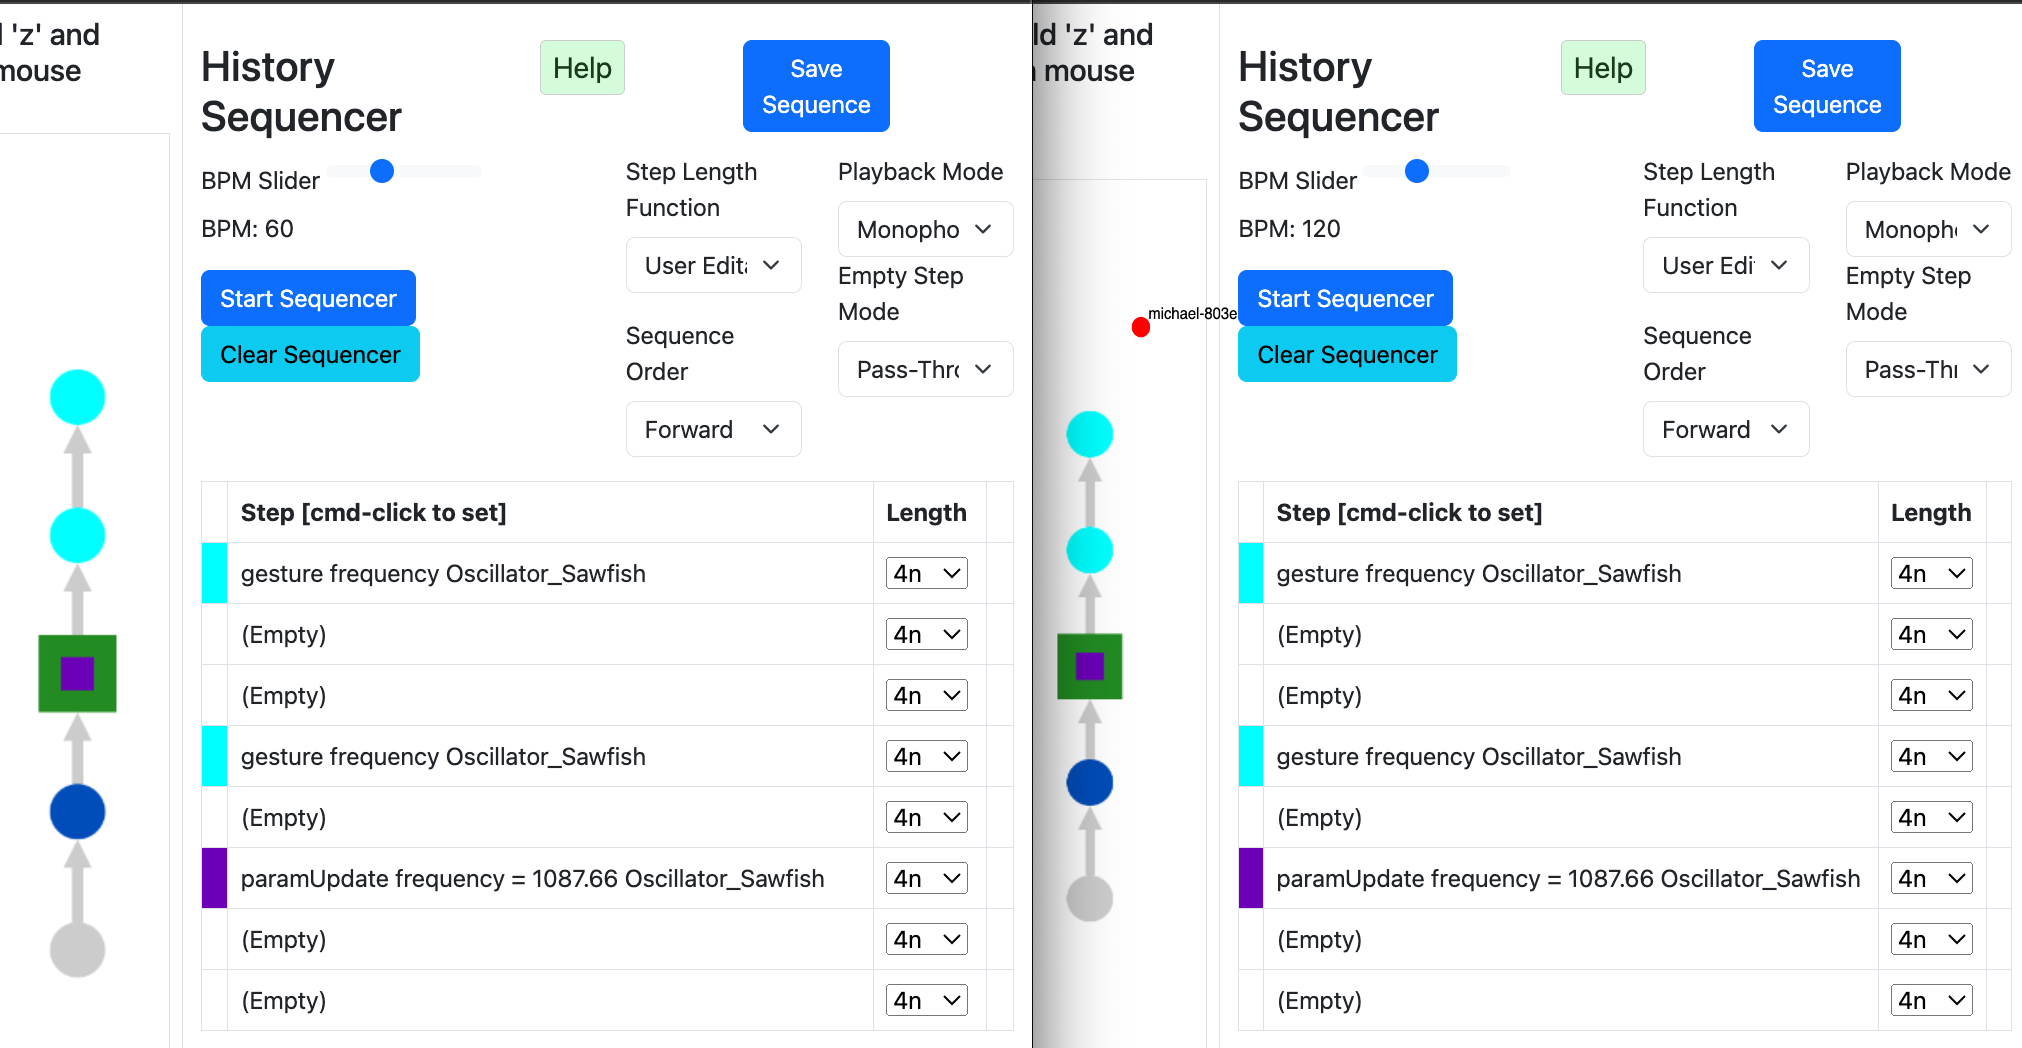
\includegraphics[width=1\linewidth]{__Figures/MP - Sequencer Syncd.png}
    \caption[Sequencer Synchronization]{Real-time sequencer sync between two Forking Paths windows, with the left player’s cursor shown as a red dot on the right.}
    \label{fig:sequencer-sync}
\end{figure}

\chapter{Evaluation and Discussion}

This chapter presents the evaluation of the research outcomes and reflects on their broader implications. Depending on the discipline, evaluation may involve user studies, expert feedback, performance documentation, case analyses, or critical reflection.  

The goals of this chapter are threefold:  
1. To provide evidence that the work achieves its intended aims.  
2. To situate the findings within wider scholarly, creative, or technical contexts.  
3. To discuss limitations and propose directions for future work.  

\section{Evaluation Methods}
Describe how the work was evaluated (e.g., user testing, critical analysis, field studies, performance documentation).  

\section{Findings}
Present the results of the evaluation in a clear and organized way. Use tables, figures, or quotations where appropriate.  

\section{Discussion}
Interpret the findings, highlight strengths and weaknesses, and connect them back to the research questions or objectives.  

\section{Future Work}
Outline potential extensions, improvements, or new research directions that build on the contributions of this dissertation.


\chapter{Conclusion}


Write your conclusion chapter here. 



%   BACK MATTER  %%%%%%%%%%%%%%%%%%%%%%%%%%%%%%%%%%%%%%%%%%%%%%%%%%%%%%%%%%%%%%
%
%   References and appendices. Appendices come after the bibliography and
%   should be in the order that they are referred to in the text.
%
%   If you include figures, etc. in an appendix, be sure to use
%
%       \caption[]{...}
%
%   to make sure they are not listed in the List of Figures.
%

\backmatter%
\printbibliography[heading=bibintoc,title={Bibliography}]

    % \addcontentsline{toc}{chapter}{Bibliography} % adds “Bibliography” to the ToC
    % % \addtoToC{Bibliography}
    % \bibliographystyle{chicago}
    % \bibliography{references}

\begin{appendices} % optional

% % playtest questions
% \include{appendix/appendix-playtest-questions}

% synthApp code fragments
\chapter{Code Excerpts from the Synth View}
\label{app:synthAppExcerpts}

\textit{Please note that this appendix was included in Michael Palumbo's dissertation. It is included here to demonstrate how to reference a section within an appendix in the main document. Search for the following text in thesis.tex for how this works: "see Listing~\ref{lst:loadVersion-function} in Appendix~\ref{app:synthAppExcerpts}"}

A selection of notable code listings from \texttt{synthApp.js}, the Script for the Synth View Window. Each excerpt is documented in this appendix, with its corresponding location in \texttt{synthApp.js} indicated in the Lines column below.

\begin{table}[h]
  \centering
  \caption[Code Excerpts: Synth View]{Code excerpts from the Synth View}
  \begin{tabular}{@{}llll@{}}
    \toprule
    \textbf{Listing} & \textbf{Excerpt} & \textbf{Purpose} & \textbf{Lines} \\
    \midrule
    \ref{lst:automerge-initialization} & startAutomerge() & Initializes Automerge documents & 691-820 \\

\ref{lst:createNewPatchHistory} & createNewPatchHistory() & Clears patch history, DSP \& Cytoscape & 1097-1274 \\

\ref{lst:applyChange-examples} & applyChange() examples & paramUpdate \& gesture changeNodes & 3536-3578 \\

\ref{lst:applyChange} & applyChange() & Manages document updates & 834-961 \\

\ref{lst:loadVersion-function} & loadVersion() & Handles changeNodes \& branching & 1505-1656 \\

\ref{lst:updateSynthWorklet-function} & updateSynthWorklet() & Handles changes to DSP &  4873-4936 \\

\ref{lst:updateCytoscapeFromDocument} & updateCytoscapeFromDocument() & Handles changes to Cytoscape synth &  1302-1405 \\

\ref{lst:createMerge-function} & createMerge() & Merges two changeNodes & 1822–1901 \\
\ref{lst:startCable-function} & startCable() & Creates a temporary cable & 5213-5255 \\
\ref{lst:handleRemoteCables-function} & handleRemoteCables() & Renders peer temporary cables & 5257–5314 \\
\ref{lst:isEdgeInCycle-function} & isEdgeInCycle() & Graph cycle detection & 5581–5703 \\
    \bottomrule
  \end{tabular}
\end{table}

\section{Automerge Initialization}

\begin{lstlisting}[language=JavaScript, caption={Initial peer setup when joining a room}, label={lst:automerge-initialization}]
let automergeRunning = false
//* AUTOMERGE IMPLEMENTATION
async function startAutomerge () {
    automergeRunning = true
    // Load Automerge asynchronously and assign it to the global variable
    Automerge = await import('@automerge/automerge');
    
    // if the room contains 2 peers:
    if(room && roomDetails.peer1 && roomDetails.peer2){
        patchHistory = Automerge.init();
        syncState = Automerge.initSyncState(); // this must exist here
        console.log("Joining active room. Waiting for sync.");
        holdSnackbar('Syncing with peers, please wait...')
        // arm the reload function. if peer connection takes too long, it will reload the page
        forceReload(true)
        return
    } else {
        const saved = await loadDocument(patchHistoryKey);
        
        if (saved) {
            patchHistory = Automerge.load(saved);
        } else {
            patchHistory = Automerge.from({
                title: "Forking Paths Synth",
                forked_from_id: null, // used by the database to either determine this as the root of a tree of patch histories, or a fork from a stored history 
                authors: [], // this will get added to as the doc is forked from the database
                branches: {},
                branchOrder: [],
                docs: {},
                head: {
                    hash: null,
                    branch: null
                } ,
                userSettings: {
                    focusNewBranch: true 
                },
                sequencer: {
                    bpm: 120,
                    ms: 500,
                    traversalMode: 'Sequential'
                },
                synth: {
                    rnboDeviceCache: null,
                }
            });
            console.log("No saved patchHistory found. Starting fresh:", patchHistoryKey);
            await saveDocument(patchHistoryKey, Automerge.save(patchHistory));
        }
    }
            
    syncState = Automerge.initSyncState()

    // * synth changes document
    docID = 'forkingPathsDoc'; // Unique identifier for the document
    // Load the document from patchHistory's store in IndexedDB or create a new one if it doesn't exist

    // currentBranch = await loadDocument(docID);
    // if patchHistory doesn't contain a document, create a new one
    if (!patchHistory.docs[patchHistory.head.branch]) {

        currentBranch = Automerge.init();

        // load synthFile from indexedDB
        // let synthFile = JSON.parse(localStorage.getItem('synthFile'))
        // console.log('synthFile', synthFile)
        if (patchHistory.synthFile) {
           
            createNewPatchHistory(patchHistory.synthFile)
            // const firstChangeLabel = synthFile.name
            // ? `load_synth:${synthFile.name}`
            // : 'load_synth:unnamed';
        
            // currentBranch = Automerge.change(currentBranch, firstChangeLabel, (currentBranch) => {
            //     currentBranch.title = config.patchHistory.firstBranchName;
            //     currentBranch.changeNode = { msg: firstChangeLabel };
            //     currentBranch.elements = synthFile.visualGraph?.elements?.nodes || [];
            //     currentBranch.synth = {
            //         graph: synthFile.audioGraph || {
            //         modules: {},
            //         connections: []
            //         }
            //     };
            //     currentBranch.sequencer = { tableData: [] };
            // });
        
            // const hash = Automerge.getHeads(currentBranch)[0];
            // previousHash = hash;
        
            // patchHistory = Automerge.change(patchHistory, (patchHistory) => {
            //     patchHistory.branches[config.patchHistory.firstBranchName] = {
            //         head: hash,
            //         root: null,
            //         parent: null,
            //         history: [{ hash: hash, parent: null, msg: firstChangeLabel }]
            //     };
            
            //     patchHistory.docs[config.patchHistory.firstBranchName] = Automerge.save(currentBranch);
            //     patchHistory.head.branch = config.patchHistory.firstBranchName;
            //     patchHistory.head.hash = hash;
            //     patchHistory.branchOrder.push(config.patchHistory.firstBranchName);
            // });

            // // send doc to history app
            // reDrawHistoryGraph()
        
        } else {
            console.log("No synth file found. currentBranch initialized but not changed.");
            previousHash = null;

            try {
                    // Fetch the Demo Synth
                const response = await fetch(`/assets/synths/${import.meta.env.VITE_FIRST_SYNTH}.fpsynth`);
                
                if (!response.ok) {
                    throw new Error(`HTTP error! status: ${response.status}`);
                }
                
                // Parse the response as JSON
                const fileContent = await response.json();
                
                // Store the JSON string in localStorage if needed
                localStorage.setItem('synthFile', JSON.stringify(fileContent));
                
                // Process the JSON content
                createNewPatchHistory(fileContent);
        
                // enable new history button now that a synth has been loaded
                // UI.menus.file.newPatchHistory.disabled = false
              
            } catch (error) {
                console.error("Error loading template file:", error);
            }
       

        
            // patchHistory = Automerge.change(patchHistory, (patchHistory) => {
            //     // Only set up empty branch patchHistorydata — no doc yet
            //     patchHistory.branches[config.patchHistory.firstBranchName] = {
            //         head: null,
            //         root: null,
            //         parent: null,
            //         history: []
            //     };
            //     patchHistory.head.branch = config.patchHistory.firstBranchName;
            //     patchHistory.head.hash = null;
            //     patchHistory.branchOrder.push(config.patchHistory.firstBranchName);
            // });
        }

    } else {

        // patchHistory does contain at least one document, so grab whichever is the one that was last looked at
        currentBranch = Automerge.load(patchHistory.docs[patchHistory.head.branch]);

        // wait 1 second before loading content (give the audio worklet a moment to load)
        setTimeout(()=>{
            updateSynthWorklet('loadVersion', currentBranch.synth.graph, null, currentBranch.type)

            updateCytoscapeFromDocument(currentBranch, 'buildUI');
            
            previousHash = patchHistory.head.hash
            
            // send doc to history app
            reDrawHistoryGraph()

            // load the draw canvas
            if(currentBranch.drawing){
                loadCanvasVersion(currentBranch.drawing)
            }

        }, 1000);
    }
}

\end{lstlisting}

\section{createNewPatchHistory()}

\begin{lstlisting}[language=JavaScript, caption={Clears the patchHistory Automerge document, clears DSP and Cytoscape.js states, reloads the current .fpSynth file as the first change in the patchHistory and redraws UI elements}, label={lst:createNewPatchHistory}]
function createNewPatchHistory(synthFile){
    // clear the pen tool interface
    resetDrawing()
    // delete the document in the indexedDB instance
    deleteDocument('patchHistory')
    // clear DSP
    updateSynthWorklet('clearGraph')
    // ensure floating UI container divs are removed
    clearparamContainerDivs()
    // clear the sequencer
    sendMsgToHistoryApp({
        appID: 'forkingPathsMain',
        cmd: 'newPatchHistory'
            
    })
    // tell server to erase the patchHistory & send a blank DAG to client(s)
    ws.send(JSON.stringify({
        cmd: 'clearHistoryGraph'
    }))

    // Clear existing elements from Cytoscape instance
    synthGraphCytoscape.elements().remove();
    
    // remove all dynamicly generated UI overlays (knobs, umenus, etc)
    removeUIOverlay('allNodes')
    // ensure their container divs are removed too
    clearparamContainerDivs()
    // init new patch history for Automerge
    let patchHistoryJSON = {
        title: "Forking Paths Patch History",
        forked_from_id: null, // used by the database to either determine this as the root of a tree of patch histories, or a fork from a stored history 
        authors: [], // this will get added to as the doc is forked from the database
        branches: {},
        branchOrder: [],
        docs: {},
        head: {
            hash: null,
            branch: config.patchHistory.firstBranchName
        },
        
        userSettings: {
            focusNewBranch:false 
        },
        sequencer: {
            bpm: 120,
            ms: 500,
            traversalMode: 'Sequential'
        },
        synth: {
            rnboDeviceCache: null,
        },

    }
    if(synthFile){
        patchHistoryJSON.synthFile = synthFile
    } else if (patchHistory.synthFile){
        // if a synth file had been previously loaded, load it again
        patchHistoryJSON.synthFile = patchHistory.synthFile
        synthFile = patchHistory.synthFile
    }
    // assign patch history to automerge
    patchHistory = Automerge.from(patchHistoryJSON)
    // clear the current automerge doc
    currentBranch = Automerge.init();

    if(synthFile || patchHistory.synthFile){

        if(!patchHistory.synthFile) { synthFile = patchHistory.synthFile }

        let amMsg = makeChangeMessage(config.patchHistory.firstBranchName, `loaded ${synthFile.filename}`)
    
        // Apply initial changes to the new document
        currentBranch = Automerge.change(currentBranch, amMsg, (currentBranch) => {
            currentBranch.title = config.patchHistory.firstBranchName;
            currentBranch.elements = [ ] 
            patchHistory.synthFile.visualGraph.elements.nodes.forEach((node)=>{
                currentBranch.elements.push(node)
            })
            
            currentBranch.synth = {
                graph: synthFile.audioGraph,
                connections: []
            }
            
            audioGraphDirty = true

            currentBranch.drawing = []
        }, onChange, `loaded ${synthFile.filename}`);

        updateSynthWorklet('loadVersion', currentBranch.synth.graph, null, currentBranch.changeNode)
        
        // load synth graph from file into cytoscape
        synthGraphCytoscape.json(patchHistory.synthFile.visualGraph)

        synthFile.visualGraph.elements.nodes.forEach((node, index)=>{
            // set module grabbable to false -- prevents module movements in main view
            if(node.classes === ':parent'){
                // synthFile.visualGraph.elements.nodes[index].grabbable = false
                // lock the module's position
                synthGraphCytoscape.getElementById(node.data.id).lock();
            }
            // create overlays
            if(node.classes === 'paramAnchorNode'){
                let value = patchHistory.synthFile.audioGraph.modules[node.data.parent].params[node.data.label]
                createFloatingOverlay(node.data.parent, node, index, value)
        
                // index++
            }
        })


        setTimeout(() => {
            updateKnobPositionAndScale('all');
            // Make all nodes non-draggable
            
        }, 10); // Wait for the current rendering cycle to complete
    } else { 
        console.log('non synthFile')
        console.warn('synthFile nor patchHistory.synthFile not found')
        
    }

    let hash = Automerge.getHeads(currentBranch)[0]
    previousHash = hash

    let msg = 'blank_patch'
    if (synthFile){
        msg = `loaded ${synthFile.filename}`
    }
    patchHistory = Automerge.change(patchHistory, (patchHistory) => {
        patchHistory.branches[config.patchHistory.firstBranchName] = {
            head: hash,
            root: null,
            parent: null,
            // doc: currentBranch,
            history: [ {hash: hash, parent: null, msg: msg} ] 
        }
        
        // encode the doc as a binary object for efficiency
        patchHistory.docs[config.patchHistory.firstBranchName] = Automerge.save(currentBranch)
        patchHistory.head.branch = config.patchHistory.firstBranchName
        patchHistory.head.hash = hash 
        patchHistory.branchOrder.push(patchHistory.head.branch)
        patchHistory.synthFile = synthFile
        
    });     
        
    docUpdated = true
    previousHash = patchHistory.head.hash
    // send doc to history app
    reDrawHistoryGraph()

    // store it in the database
    const patch_binary = fromByteArray(Automerge.save(patchHistory))
    ws.send(JSON.stringify({
        cmd: 'newPatchHistory',
        data: {
            name: `${chance.animal()} ${uuidv7().split('-')[2]}`,
            authors: [ thisPeerID ],
            description: null,
            modules: ['test'], // can be pulled from your patch graph
            synth_template: patchHistory.synthFile, // JSON object
            patch_binary: patch_binary, // base64-encoded string
            forked_from_id: patchHistory.forked_from_id, // or null if this is a root version
        }
    }))

    // get a binary from the new patchHistory
    const fullBinary = Automerge.save(patchHistory);
    // send it to any connected peer(s)
    let message = {
        cmd: 'replacePatchHistory',
        data: fromByteArray(fullBinary)  // base64 encoded or send as Uint8Array directly if channel supports it
    }
    // sync with peer(s)
    sendDataChannelMessage(message)
}

\end{lstlisting}

\section{applyChange Examples}
% NOTE: this is already being referenced in the FP chapter, so we need to make sure it is documented here!

\begin{lstlisting}[language=JavaScript, caption={Creates a new changeNode, updates the DSP graph, adds both to the patch history. There are many instances of this throughout the synthApp.js, and the method for creating paramUpdate or gesture changeNodes is what is documented here.}, label={lst:applyChange-examples}]
// Listen for mouse up event on the document
document.addEventListener('mouseup', function(event) {
    hid.mouse.left = false
    
    // if the player has been playing with a param knob, we need to store it in automerge
    if(Object.keys(groupChange).length > 0){
        // if we are storing a single param change, do a paramUpdate
        if(groupChange.values.length === 1){
            // Update in Automerge
            currentBranch = applyChange(currentBranch, (currentBranch) => {
                // update DSP
                currentBranch.synth.graph.modules[groupChange.parentNode].params[groupChange.paramLabel] = groupChange.values[0];
                audioGraphDirty = true;
                // set the changeNode
                currentBranch.changeType = {
                    msg: 'paramUpdate',
                    param: groupChange.paramLabel,
                    parent: groupChange.parentNode,
                    value: groupChange.values
                }
            }, onChange, `paramUpdate ${groupChange.paramLabel} = ${groupChange.values[0]}$PARENT ${groupChange.parentNode}`);

        } else if(groupChange.values.length > 1){
            // are storing a gesture
            // Update in Automerge
            currentBranch = applyChange(currentBranch, (currentBranch) => {
                currentBranch.synth.graph.modules[groupChange.parentNode].params[groupChange.paramLabel] = groupChange.values;
                audioGraphDirty = true;
                // set the change type
                currentBranch.changeType = {
                    msg: 'gesture',
                    param: groupChange.paramLabel,
                    parent: groupChange.parentNode,
                    values: groupChange.values,
                    timestamps: groupChange.timestamps
                }
            }, onChange, `gesture ${groupChange.paramLabel}$PARENT ${groupChange.parentNode}`);

        }

        // clear the groupChange
        groupChange = { }
    }

    // ... rest of code omitted for brevity
});

\end{lstlisting}



\section{applyChange}

\begin{lstlisting}[language=JavaScript, caption={applyChange() manages Automerge document updates within Forking Paths. If the user is working on the current branch, the function applies changes directly and appends a new commit to that branch’s history. If the user is editing a past state (i.e., newClone is true), the function forks a new branch, applies the change, and updates the patch history metadata accordingly. In both cases, the current Automerge document is saved, a new hash is generated, and the onChangeCallback is triggered to sync peers, update the UI, and redraw the version history graph.}, label={lst:applyChange}]
// handle document changes and call a callback
function applyChange(doc, changeCallback, onChangeCallback, changeMessage) {
    // in this condition, we are applying a change on the current branch
    if(automergeDocuments.newClone === false ){
        let amMsg = makeChangeMessage(patchHistory.head.branch, changeMessage)
        // we are working from a head

        // grab the current hash before making the new change:
        previousHash = patchHistory.head.hash
        
        // Apply the change using Automerge.change
        currentBranch = Automerge.change(currentBranch, amMsg, changeCallback);


        // If there was a change, call the onChangeCallback
        if (currentBranch !== doc && typeof onChangeCallback === 'function') {
            let hash = Automerge.getHeads(currentBranch)[0]
            
            patchHistory = Automerge.change(patchHistory, (patchHistory) => {

                // if the current patchHistory was loaded from the database, then we need to create a fork for this new change
                if (patchHistory.hasBeenModified === false) {
                    patchHistory.forked_from_id = patchHistory.databaseID
                    patchHistory.hasBeenModified = true
                    forkHistoryInDatabase(patchHistory.databaseID)
                }
                // Initialize the branch patchHistorydata if it doesn't already exist
                if (!patchHistory.branches[patchHistory.head.branch]) {
                    patchHistory.branches[patchHistory.head.branch] = { head: null, history: [] };
                }
                // Update the head property
                patchHistory.branches[patchHistory.head.branch].head = hash;

                // Push the new history entry into the existing array
                patchHistory.branches[patchHistory.head.branch].history.push({
                    hash: hash,
                    parent: previousHash,
                    msg: changeMessage,
                    timeStamp: new Date().getTime()

                });

                // encode the doc as a binary object for efficiency
                patchHistory.docs[patchHistory.head.branch] = Automerge.save(currentBranch)
                // store the HEAD info
                patchHistory.head.hash = hash
                patchHistory.timeStamp = new Date().getTime()
                //? patchHistory.head.branch = currentBranch.title
                
            });


            
            updatePatchHistoryDatabase()

            onChangeCallback(currentBranch);
        }
        return currentBranch;
    } else {
        // player has made changes to an earlier version, so create a branch and set currentBranch to new clone

        // store previous currentBranch in automergeDocuments, and its property is the hash of its head
        automergeDocuments.otherDocs[patchHistory.head.branch] = currentBranch
        // set currentBranch to current cloned doc
        currentBranch = Automerge.clone(automergeDocuments.current.doc)

        // create a new branch name
        const newBranchName = uuidv7();
        // use the new branch title
        let amMsg = makeChangeMessage(patchHistory.head.branch, changeMessage)

        // grab the current hash before making the new change:
        previousHash = Automerge.getHeads(currentBranch)[0]
        
        // Apply the change using Automerge.change
        currentBranch = Automerge.change(currentBranch, amMsg, changeCallback);
        let hash = Automerge.getHeads(currentBranch)[0]
        
        // If there was a change, call the onChangeCallback
        if (currentBranch !== doc && typeof onChangeCallback === 'function') {   
            const timestamp = new Date().getTime()
            patchHistory = Automerge.change(patchHistory, (patchHistory) => {

                // create the branch
                patchHistory.branches[newBranchName] = {
                    head: hash,
                    parent: previousHash,
                    history: [{
                        hash: hash,
                        msg: changeMessage,
                        parent: previousHash,
                        timeStamp: timestamp
                    }]
                }

                // store current doc
                patchHistory.docs[newBranchName] = Automerge.save(currentBranch)
                
                // store the HEAD info
                patchHistory.head.hash = hash
                patchHistory.head.branch = newBranchName

                patchHistory.timeStamp = timestamp

                // store the branch name so that we can ensure its ordering later on
                patchHistory.branchOrder.push(newBranchName)

                // if the current patchHistory was loaded from the database, then we need to create a fork for this new change
                if (patchHistory.hasBeenModified === false) {
                    patchHistory.forked_from_id = patchHistory.databaseID
                    patchHistory.hasBeenModified = true
                    forkHistoryInDatabase(patchHistory.databaseID)
                }
            });
           
            // makeBranch(changeMessage, Automerge.getHeads(newDoc)[0])
            onChangeCallback(currentBranch);

            updatePatchHistoryDatabase()
            automergeDocuments.newClone = false

        }
        return currentBranch;

    }
    

}

    // define the onChange Callback
    onChange = () => {
        // send to peer(s)
        sendSyncMessage()
        // set docUpdated so that indexedDB will save it
        docUpdated = true
        // update the historyGraph in the server
        reDrawHistoryGraph()
        // set audioDirty flag
        if(audioGraphDirty){
            audioGraphDirty = false
    }
};

\end{lstlisting}

\section{loadVersion()}

\begin{lstlisting}[language=JavaScript, caption={The loadVersion() function loads a specific changeNode from the patch history when a player selects it in the DAG, restoring the associated synth configuration and patch history sequencer state using the provided branch name and hash.}, label={lst:loadVersion-function}]
// Load a version from the DAG
async function loadVersion(targetHash, branch, fromPeer, fromPeerSequencer) {
    // get the head from this branch
    let head = patchHistory.branches[branch].head
    // get the automerge doc associated with the requested hash
    let requestedDoc = loadAutomergeDoc(branch)
    // Use `Automerge.view()` to view the state at this specific point in history
    const historicalView = Automerge.view(requestedDoc, [targetHash]);
    // load the pen tool drawing
    if(historicalView.drawing){
        loadCanvasVersion(historicalView.drawing)
    }
    
    // Check if we're on the head; reset clone if true (so we don't trigger opening a new branch with changes made to head)
    // compare the point in history we want (targetHash) against the head of its associated branch (head)
    if (head === targetHash){

        // no need to create a new branch if the user makes changes after this operation
        automergeDocuments.newClone = false
        // send the synth graph from this point in the history to the DSP worklet first
        updateSynthWorklet('loadVersion', historicalView.synth.graph)
        // send the visual graph from this point in the history to the synth cytoscape
        updateCytoscapeFromDocument(historicalView);
        // update patchHistory to set the current head and change hash
        patchHistory = Automerge.change(patchHistory, (patchHistory) => {
            // store the HEAD info (the most recent HEAD and branch that were viewed or operated on)
            patchHistory.head.hash = targetHash
            patchHistory.head.branch = branch
        });
        // set global var for easy checking
        automergeDocuments.current = {
            doc: requestedDoc
        }        
    } 
    // this is necessary for loading a hash on another branch that ISN'T the head
    else if (branch != patchHistory.head.branch) {

        // if we are dealing with a blank patch, then clear the audio graph
        if(!historicalView.synth){
            updateSynthWorklet('clearGraph')
        } else {
            // send the synth graph from this point in the history to the DSP worklet first
            updateSynthWorklet('loadVersion', historicalView.synth.graph, null, historicalView.changeType)
        }

        // send the visual graph from this point in the history to the synth cytoscape
        updateCytoscapeFromDocument(historicalView);
        // set global var for easy checking
        automergeDocuments.current = {
            doc: requestedDoc
        }
        // update patchHistory to set the current head and change hash
        patchHistory = Automerge.change(patchHistory, (patchHistory) => {
            // store the HEAD info (the most recent HEAD and branch that were viewed or operated on)
            patchHistory.head.hash = targetHash
            patchHistory.head.branch = branch
        });
        // set newClone to true
        automergeDocuments.newClone = true
    }
    // the selected hash belongs to the current branch
    else {
        // send the synth graph from this point in the history to the DSP worklet first
        updateSynthWorklet('loadVersion', historicalView.synth.graph, null, historicalView.changeType)
        // send the visual graph from this point in the history to the synth cytoscape
        updateCytoscapeFromDocument(historicalView);
        // create a clone of the branch in case the player begins making changes
        let clonedDoc = Automerge.clone(historicalView)
        // store it
        automergeDocuments.current = {
            doc: clonedDoc
        }
        // set newClone to true
        automergeDocuments.newClone = true

        // update patchHistory to set the current head and change hash
        patchHistory = Automerge.change(patchHistory, (patchHistory) => {
            // store the HEAD info (the most recent HEAD and branch that were viewed or operated on)
            patchHistory.head.hash = targetHash
            patchHistory.head.branch = branch
        });
    }

    // Optional sync/permission handling AFTER local load
    const recallMode = getVersionRecallMode();
    // ensure that loadVersion calls from the peer don't make past this point, becuase otherwise they'd send it back and forth forever 
    if (recallMode === 'openLoadVersion' && !fromPeer && !fromPeerSequencer) {
        console.log('openVersionRecall')
        openVersionRecall(targetHash, branch);
    }

    if (recallMode === 'requestOpenLoadVersion'  && !fromPeer) {
        // requestVersionRecallWithPermission(currentBranch, Automerge.getHeads(currentBranch)[0], patchHistory.head.branch);
        console.warn('not set up yet')
    }

} 
\end{lstlisting}


\section{updateSynthWorklet()}

\begin{lstlisting}[language=JavaScript, caption={Sends commands from the UI to the synthWorklet audio engine via the Web Audio API’s message port. Supports graph updates (e.g., adding/removing nodes or cables), parameter changes, and signal analysis configuration. Commands are structured and dispatched using a switch statement.}, label={lst:updateSynthWorklet-function}]
function updateSynthWorklet(cmd, data, structure, changeNode){

    switch (cmd) {
        case 'setOutputVolume':
            synthWorklet.port.postMessage({ 
                cmd: 'setOutputVolume',
                data: data
            });
        break
        case 'clearGraph':
            synthWorklet.port.postMessage({ 
                cmd: 'clearGraph'
            });
        break
        case 'loadVersion':
            synthWorklet.port.postMessage({ 
                cmd: 'loadVersion', 
                data: data,
            });
        break

        case 'setSignalAnalysis':
            synthWorklet.port.postMessage({ 
                cmd: 'setSignalAnalysis', 
                data: data
            });
        break
        
        case 'addNode':
            synthWorklet.port.postMessage({ 
                cmd: 'addNode', 
                data: data,
                structure: structure
            });
        break

        case 'removeNode':
            synthWorklet.port.postMessage({ 
                cmd: 'removeNode', 
                data: data
            });
        break

        case 'addCable':
            synthWorklet.port.postMessage({
                cmd: 'addCable',
                data: data
            });

        break

        case 'removeCable':
            synthWorklet.port.postMessage({
                cmd: 'removeCable',
                data: data
            });
        break

        case 'paramChange':

            synthWorklet.port.postMessage({ cmd: 'paramChange', data: data });
        break
    }

}
\end{lstlisting}

\section{updateCytoscapeFromDocument()}

\begin{lstlisting}[language=JavaScript, caption={The updateCytoscapeFromDocument() function rebuilds the visual patch graph in Cytoscape.js based on a loaded changeNode document. It supports three modes: buildUI is triggered after loading a .fpsynth synthesizer file and fully reconstructs the interface, including parameter overlays. The default mode responds to changes or version loads initiated by the local player, while buildFromSyncMessage applies state changes received from a remote peer. Since rebuilding UI overlays involves additional computation, the latter two modes skip this step unless overlays are missing and must be regenerated.}, label={lst:updateCytoscapeFromDocument}]
// Function to update Cytoscape with the state from the loaded changeNode doc (referred to here as 'forkedDoc')
function updateCytoscapeFromDocument(forkedDoc, cmd, lastGestureValue) {
    App.synth.visual.modules = forkedDoc.synth.graph.modules
    let elements = forkedDoc.elements
    peers.remote = {}
    // only rebuild the UI if needed
    if(cmd === 'buildUI'){
        parentNodePositions = []; // Array to store positions of all parent nodes

        // Step 1: Extract all parent nodes from the given document
        const parentNodes = forkedDoc.elements.filter(el => el.classes === ':parent'); // Adjust based on your schema
        parentNodes.forEach(parentNode => {
            if (parentNode.position) {
                parentNodePositions.push({
                    id: parentNode.data.id,
                    position: parentNode.position
                });
            }
        })
        
        // Clear existing elements from Cytoscape instance
        synthGraphCytoscape.elements().remove();

        // remove all dynamicly generated UI overlays (knobs, umenus, etc)
        removeUIOverlay('allNodes')
        
        // ensure their container divs are removed too
        clearparamContainerDivs()

        // I do this from the synthFile because the parentNodes' dimensions respond to their childs' positioning
        synthGraphCytoscape.json(patchHistory.synthFile)
        // synthGraphCytoscape.nodes(':parent').forEach(n => console.log(n.id())); // lock all parent nodes so they can't be dragged
        // Sync the positions in `elements`
        const syncedElements = syncPositions(forkedDoc);
        // add all cables back in with a check to make sure we don't render edges to empty parent nodes
        for (let i = 0; i < syncedElements.length; i++) {
            const el = syncedElements[i];
            if (el.type === 'edge') {
                const sourceExists = synthGraphCytoscape.getElementById(el.data.source).length > 0;
                const targetExists = synthGraphCytoscape.getElementById(el.data.target).length > 0;

                if (!sourceExists || !targetExists) {
                    console.warn(`Skipping edge: ${el.data.id} due to missing source or target`);
                    continue; // Skip this iteration and move to the next element
                }
            }

            synthGraphCytoscape.add(el);
        }
        
        let index = 0
        elements.forEach((node)=>{
            // set module grabbable to false -- prevents module movements in main view
            if(node.classes === ':parent'){
                // lock the module's position
                synthGraphCytoscape.getElementById(node.data.id).lock();
            }
            if(node.classes === 'paramAnchorNode'){
                let value = App.synth.visual.modules[node.data.parent].params[node.data.label]
                createFloatingOverlay(node.data.parent, node, index, value)
                index++
            }
        })
        // Initial position and scale update. delay it to wait for cytoscape rendering to complete. 
        setTimeout(() => {
            updateKnobPositionAndScale('all');
        }, 10); // Wait for the current rendering cycle to complete
        
        // After loading your synth and creating overlays:
        cacheVisibleParamControls(App.synth.visual.modules);
        
    } else if (cmd === 'buildFromSyncMessage'){
        // Sync the positions in `elements`
        const syncedElements = syncPositions(forkedDoc);
        // clear 
        synthGraphCytoscape.elements().remove();

        // 3. Add new elements to Cytoscape
        synthGraphCytoscape.add(syncedElements)

        // check to see if none of the overlays were made. this is the case if peer has a blank document and is syncing to another peer's doc
        const overlaysExist = document.querySelector('[id^="paramControl_parent:"]') !== null;

        if (!overlaysExist) {
            updateCytoscapeFromDocument(forkedDoc, 'buildUI');
            return; // skip the rest, since buildUI handles everything
        }

        refreshParamControls(App.synth.visual.modules, lastGestureValue);
    }
    
    
    else {
        // Sync the positions in `elements`
        const syncedElements = syncPositions(forkedDoc);
        // clear 
        synthGraphCytoscape.elements().remove();

        // 3. Add new elements to Cytoscape
        synthGraphCytoscape.add(syncedElements)

        refreshParamControls(App.synth.visual.modules);
    }
}   

\end{lstlisting}





\section{createMerge()}

\begin{lstlisting}[language=JavaScript, caption={The createMerge function takes two changeNodes selected by the player and merges them. A new branch is created to store the result of the merge. The unified patch state is then loaded into the main application and rendered in the visual and audio synth graphs.}, label={lst:createMerge-function}]
// merge 2 versions & create a new node in the history graph
function createMerge(nodes){
    let doc1 = nodes[0]
    let doc2 = nodes[1]

    // load historical views of both docs
    let requestedDoc1 = loadAutomergeDoc(doc1.branch)
    let requestedDoc2 = loadAutomergeDoc(doc2.branch)
    // merge them
    let mergedDoc = Automerge.merge(requestedDoc1, requestedDoc2)
    let hashes = [ doc1.id, doc2.id ]

    // create empty change to 'flatten' the merged Doc
    currentBranch = Automerge.emptyChange(mergedDoc);

    let hash = Automerge.getHeads(currentBranch)[0]
    // make new branch name
    const newBranchName = uuidv7()
    // update the patchHistory in Automerge
    patchHistory = Automerge.change(patchHistory, { message: `merge parents: ${doc1.id} ${doc2.id} `}, (patchHistory) => {
        // Initialize the branch patchHistorydata if it doesn't already exist
        if (!patchHistory.branches[newBranchName]) {
            patchHistory.branches[newBranchName] = { 
                head: null, 
                parent: [ doc1.id, doc2.id ], 
                history: [] 
            };           
        }
        // Update the head property
        patchHistory.branches[newBranchName].head = hash;
        // Push the new history entry into the existing array
        patchHistory.branches[newBranchName].history.push({
            hash: hash,
            msg: 'merge',
            parent: hashes,
            nodes: [doc1, doc2]
        });
        // store current doc
        patchHistory.docs[newBranchName] = Automerge.save(currentBranch)        
        // store the HEAD info
        patchHistory.head.hash = hash
        patchHistory.head.branch = newBranchName
        // store the branch name so that we can ensure its ordering later on
        patchHistory.branchOrder.push(newBranchName)
    });
    // set docUpdated so that indexedDB will save it
    docUpdated = true
    // update the audio graph
    updateSynthWorklet('loadVersion', currentBranch.synth.graph)
    // update the synth graph (visual)
    updateCytoscapeFromDocument(currentBranch, 'buildUI');
    // update the historyGraph
    reDrawHistoryGraph()
}
\end{lstlisting}

\section{startCable()}
\begin{lstlisting}[language=JavaScript, caption={Function startCable() creates a temporary visual connection between a source node and the mouse position. A ghost node and dashed cable are rendered to indicate an in-progress patching action.}, label={lst:startCable-function}]
function startCable(source, position){
    temporaryCables.local.source = source;
    const mousePos = position;

    // Get the ghostCable property from the temporaryCables.local.ghostNode, default to 'ellipse' if undefined
    const ghostShape =  temporaryCables.local.source.data('ghostCableShape') || 'ellipse';
    const ghostColour =  temporaryCables.local.source.data('ghostCableColour') || '#5C9AE3';

    // Create a ghost node at the mouse position to act as the moving endpoint
    temporaryCables.local.ghostNode = synthGraphCytoscape.add({
        group: 'nodes',
        data: { id: 'localGhostNode' },
        position: mousePos,
        grabbable: false, // Ghost node shouldn't be draggable
        classes: 'ghostNode'
    });

    // Apply the ghostShape to the ghostNode using a direct style override
    temporaryCables.local.ghostNode.style({
        'shape': ghostShape,
        'background-color': ghostColour
    });
    // Create a temporary edge from ghostNodes.local.source to temporaryCables.local.ghostNode
    temporaryCables.local.tempEdge = synthGraphCytoscape.add({
        group: 'edges',
        data: { id: 'localTempEdge', source: temporaryCables.local.source.id(), target: 'localGhostNode' },
        classes: 'tempEdge'
    });

    // Set target endpoint to mouse position initially
    temporaryCables.local.tempEdge.style({ 'line-color': '#FFA500', 'line-style': 'dashed',  'source-arrow-shape': 'none'  }); // Set temporary edge color        
}
\end{lstlisting}

\section{handleRemoteCables()}
\begin{lstlisting}[language=JavaScript, caption={Handles the rendering of temporary cables created by a remote peer, updating their position in real time. These updates are transmitted over a WebRTC data channel and are intentionally kept outside the Automerge sync protocol to avoid polluting the version history.}, label={lst:handleRemoteCables-function}]
function handleRemoteCables(cmd,  peerID, sourceID, position){   
    switch(cmd){    
        case 'startRemoteGhostCable':
            let ghostId = `ghostNode-${peerID}`
            let tempEdgeID = `tempEdge-${peerID}`
            
            temporaryCables.peers[peerID] = {
                source: synthGraphCytoscape.getElementById(sourceID),
                // Create a ghost node at the mouse position to act as the moving endpoint
                ghostNode: synthGraphCytoscape.add({
                    group: 'nodes',
                    data: { id: ghostId },
                    position: position,
                    grabbable: false, // Ghost node shouldn't be draggable
                    classes: 'ghostNode'
                }),
                // Create a temporary edge from temporaryCables.local.source to ghostNode
                tempEdge: synthGraphCytoscape.add({
                    group: 'edges',
                    data: { id: tempEdgeID, source: sourceID, target: ghostId },
                    classes: 'tempEdge'
                }),
                targetNode: null
            }
            
            // set ghostNode Style according to opposite of source Node
            const ghostShape = temporaryCables.peers[peerID].source.data('ghostCableShape') || 'ellipse';
            const ghostColour = temporaryCables.peers[peerID].source.data('ghostCableColour') || '#5C9AE3';
            temporaryCables.peers[peerID].ghostNode.style({
                'shape': ghostShape,
                'background-color': ghostColour
            });

            temporaryCables.peers[peerID].tempEdge.style({ 'line-color': '#228B22', 'line-style': 'dashed', 'source-arrow-shape': 'none' }); // Set peer temporary edge color
        break;

        case 'updateRemoteGhostCable':
            // update the tmporary cable's position
            temporaryCables.peers[peerID].ghostNode.position(position)
        break

        case 'finishRemoteGhostCable':
            // remove the tempEdge
            synthGraphCytoscape.remove(temporaryCables.peers[peerID].tempEdge)
            // remove remote ghostnode
            synthGraphCytoscape.remove(temporaryCables.peers[peerID].ghostNode);
            synthGraphCytoscape.nodes().removeClass('highlighted');

            // remove remote peer's temporary cable from object
            delete temporaryCables.peers[peerID]

        break;
    }
} 

\end{lstlisting}

\section{isEdgeInCycle()}

\begin{lstlisting}[language=JavaScript, caption={Determines whether a given cable (edge) introduces a cycle in the patch graph rendered by Cytoscape. The function checks for both self-loop cycles and inter-node cycles using depth-first search (DFS). If a cycle is detected, it inserts a feedbackDelayNode with a fixed delay of 128 samples into the audio graph to allow feedback patching.}, label={lst:isEdgeInCycle-function}]
function isEdgeInCycle(edgeToCheck) {
    const parentEdges = new Map();
    const selfLoopEdges = []; // Store self-loop edges for same parent connections

    // Step 1: Build a directed graph of parent nodes with child information
    synthGraphCytoscape.edges().forEach((edge) => {
        const sourceParent = edge.data().source.split('.')[0]; // Parent of the source node
        const targetParent = edge.data().target.split('.')[0]; // Parent of the target node
        const sourceChild = edge.data().source.split('.')[1]; // Source child
        const targetChild = edge.data().target.split('.')[1]; // Target child

        if (targetParent.includes('AudioDestination')) {
            return; // Ignore connections to the audio destination
        }

        if (sourceParent === targetParent) {
            // Detect self-loop: connections within the same parent node
            selfLoopEdges.push({
                sourceParent,
                targetParent,
                sourceChild,
                targetChild,
            });
        } else {
            // Add normal inter-parent edges
            if (!parentEdges.has(sourceParent)) {
                parentEdges.set(sourceParent, []);
            }
            parentEdges.get(sourceParent).push({
                targetParent,
                sourceChild,
                targetChild,
            });
        }
    });

    // Step 2: Detect self-loop cycles
    const selfLoopMatch = selfLoopEdges.some(
        (edge) =>
            edge.sourceParent === edgeToCheck.data().source.split('.')[0] &&
            edge.targetParent === edgeToCheck.data().target.split('.')[0] &&
            edge.sourceChild === edgeToCheck.data().source.split('.')[1] &&
            edge.targetChild === edgeToCheck.data().target.split('.')[1]
    );

    if (selfLoopMatch) {
        // console.log(
        //     `Edge ${edgeToCheck.id()} forms a self-loop cycle within ${edgeToCheck.data().source.split('.')[0]}`
        // );
        return true;
    }

    // Step 3: Detect inter-parent cycles using Depth-First Search (DFS)
    const visited = new Set();
    const recStack = new Set();
    let edgeInCycle = false;

    function dfs(node, path = [], edgePath = []) {
        if (!visited.has(node)) {
            visited.add(node); // Mark the node as visited
            recStack.add(node); // Add the node to the recursion stack

            const neighbors = parentEdges.get(node) || [];
            for (const neighbor of neighbors) {
                const currentEdge = {
                    sourceParent: node,
                    targetParent: neighbor.targetParent,
                    sourceChild: neighbor.sourceChild,
                    targetChild: neighbor.targetChild,
                };

                if (!visited.has(neighbor.targetParent)) {
                    if (
                        dfs(
                            neighbor.targetParent,
                            [...path, node],
                            [...edgePath, currentEdge]
                        )
                    ) {
                        return true; // Cycle detected
                    }
                } else if (recStack.has(neighbor.targetParent)) {
                    // Cycle detected: back edge
                    const cycleStartIndex = path.indexOf(neighbor.targetParent);
                    const cycleEdges = [
                        ...edgePath.slice(cycleStartIndex),
                        currentEdge,
                    ]; // Edges in the cycle

                    // Check if the edgeToCheck belongs to this cycle
                    if (
                        cycleEdges.some(
                            (edge) =>
                                edge.sourceParent ===
                                    edgeToCheck.data().source.split('.')[0] &&
                                edge.targetParent ===
                                    edgeToCheck.data().target.split('.')[0] &&
                                edge.sourceChild ===
                                    edgeToCheck.data().source.split('.')[1] &&
                                edge.targetChild ===
                                    edgeToCheck.data().target.split('.')[1]
                        )
                    ) {
                        edgeInCycle = true;
                        return true;
                    }
                }
            }
        }

        recStack.delete(node);
        return false;
    }

    for (const node of parentEdges.keys()) {
        if (!visited.has(node)) {
            dfs(node);
            if (edgeInCycle) break; // Exit early if the edge is found in a cycle
        }
    }

    return edgeInCycle; // Return true if the edge belongs to any cycle
}


\end{lstlisting}






\bigskip
\textbf{Complete File} — The full, commented source is archived at
\\https://github.com/michaelpalumbo/forkingpaths/blob/dissertationJune/src/scripts\\/synthApp.js

% patchHistory code fragments
% \include{appendix/appendix-patchHistoryExcerpts.tex}

% Server.js
% \include{appendix/appendix-server}

% % BuildHistoryGraph.js
% \include{appendix/appendix-buildHistoryGraph}

% % DSP audioWorklet
% \include{appendix/appendix-customDSP}

% % Modules Spec
% \include{appendix/appendix-moduleSpec}

% % .fpsynth File
% \include{appendix/appendix-fpsynthFile}

% % config file
% \include{appendix/appendix-config}



\end{appendices}

\end{document}
